\documentclass{article}

\newlength\tempindent
\setlength{\tempindent}{\parindent}
\setlength{\parindent}{0pt}
\renewcommand{\indent}{\hspace*{\tempindent}}

\usepackage{multicol, amsmath, graphicx, datetime2, fancyhdr, listings, courier}
\usepackage[letterpaper, portrait, margin=1in]{geometry}
\usepackage[parfill]{parskip}

\newcommand{\subscript}[1]{$_{\text{#1}}$}
\newcommand{\mymod}[1]{\text{ } ( \text{mod } #1 )}
\newcommand{\divides}{\text{ } | \text{ }}
\newcommand{\formsep}{\indent \Big\rvert \indent}
\renewcommand{\labelitemii}{$^{\circ}$}
\newcommand*{\myfont}{\fontfamily{pcr}\selectfont}
\DeclareTextFontCommand{\inline}{\myfont}

\lstset{
	language=Java,
	basicstyle=\ttfamily,
	numbers=left,
	numberstyle=\small,
	tabsize=4,
	columns=flexible,
	showstringspaces=false,
	showtabs=false,
	keepspaces
}

\newcommand{\thetitle}{Hack Pack}
\renewcommand*{\addcontentsline}[3]{\addtocontents{#1}{\protect\contentsline{#2}{#3}{}}}
\renewcommand{\headrulewidth}{0pt}
\newcommand{\startsection}[1]{\addcontentsline{toc}{section}{#1}\section*{#1}\setcounter{page}{1}\pagestyle{fancy}\fancyhf{}\rhead{#1 \thepage}}

\title{\thetitle}
\author{Matthew Garrison}
\date{\today}

\begin{document}
\maketitle
\begin{multicols}{2}
    \tableofcontents
\end{multicols}

\newpage

\startsection{Approaches and checklist}

\textbf{Checklist of stupid mistakes}

\indent BitSets allocate memory as-needed, so you can get an \inline{OutOfBounds} exception if the index you're checking doesn't exist yet. \\
\indent Don't compare two \inline{Integers} with \inline{==}. This will work for values on $[-128, 127]$ because of caching, but will fail for values outside that range. (As long as at least one variable is an \inline{int}, you can use \inline{==}.) \\
\indent FFT: The polynomial must be \textit{exactly} the one you wish to use. For example, if you are raising a polynomial to the k\textsuperscript{th} power, and you only care about indexes less than 50000, you must zero out all the indexes past 50000, every time you multiply. \\
\indent Infinity must be sufficiently large. \\
\indent Make sure you typed the sample data correctly. \\
\indent Memo table: checking the memo table at the start of the method, storing answers in the memo table before you return them, using the right indexes (ie. the current index, not \inline{n}). \\
\indent New line in \inline{printf()}. \\ 
\indent TreeSets can sometimes have a better in-practice runtime than HashSets. 

\textbf{Feasibility}

1 second: $\leq 10^8$ operations \indent\indent
5 seconds: $\leq 10^9$ operations

Approximate size-to-runtime relationships:
\begin{itemize}
    \item $n \geq 10^7$: O($n$)
    \item $n = [10^5, 10^6]$: O($n\text{ log}(n)$)
    \item $n = 10^4$: O($n^2$)
    \item $n = 10^3$: O($n^3$)
\end{itemize}

Stack size: it varies, but generally $\leq 5000$ method calls.

Memory: $\leq 5*10^7$

Bipartite matching works on sparse graphs, V $\leq$ 5000. \\
Floyd-Warshal works on sparse and dense graphs, V $\leq$ 500. \\
Dijkstra’s works on sparse and dense graphs, V $\leq$ 5000. \\
Toposort works on sparse graphs, V $\leq$ 100,000.

\textbf{Techniques} \\ 
Meet in the middle \\
Can we eliminate a dimension of the memo table? \\
Can we not consider some cases of the DP? \\
Can we prune enough of the graph? \\
Pre-compute functions (eg. trig functions) outside of the loop, when possible 

\textbf{Test case generation} \\
Minimum sized case \\
Maximum sized case \\
Case that is specifically omitted from the sample \\
Case where 1 item that is true of average cases doesn't hold \\
Case with maximal answer \\
Case with minimal answer \\
Cases that test each line of code \\
Cases that check overflow of intermediate computations \\
Cases that check array out of bounds

\newpage
\startsection{Binary and ternary search}

\subsection*{Binary search}

\textit{Runtime: O(log(n))}

A binary search will search through an increasing or decreasing function or \underline{sorted} array for a desired value.

\lstinputlisting{general/code/binternsearch1.java}

If the array contains multiple occurrences of the value, this will find the first one. To find the last occurrence, change line \#7 to be lo = mid + 1.

\lstinputlisting{general/code/binternsearch2.java}

Binary search for the last \inline{true} value. To search for the first \inline{true}, negate the if-statement. The answer is at \inline{lo-1}.

\lstinputlisting{general/code/binternsearch3.java}

You can also search with \inline{compareTo()}:

\lstinputlisting{general/code/binternsearch4.java}

You can also do a binary search on floating point numbers. Basically, you go for repetition, instead of checking if lo exceeds hi. This is most often used when binary searching a function. The number of repetitions you need varies depending on the problem, but 100 is often enough. Make sure to stay within the time limit.

\lstinputlisting{general/code/binternsearch5.java}

Alternatively (answer at \inline{lo}):

\lstinputlisting{general/code/binternsearch6.java}

\subsection*{Ternary search}

A ternary search will find the lowest or highest value in a parabolic function. Like when using a binary search on floating points numbers, we go for repetition. Answer is at \inline{low}.

\lstinputlisting{general/code/binternsearch7.java}

Ternary search on integers:

\lstinputlisting{general/code/binternsearch8.java}

\newpage

\startsection{Bits}

\textbf{NOT}: Because Java uses two's complement, \inline{\textasciitilde n} returns \inline{abs(n) - 1}

\textbf{Left shift}: left shift of x by y is equivalent to multiplying x by 2\textsuperscript{y}

\textbf{Right shift}: right shift of x by y is equivalent to dividing x by 2\textsuperscript{y}

\textbf{Modding by a power of two}: If y = 2\textsuperscript{n}, then \inline{x \% y} is equivalent to \inline{x \& (y - 1)}

\textbf{Check if \inline{n} is a power of two}: \inline{n != 0 \&\& (n \& (n - 1)) == 0}

Alternatively: \inline{Integer.bitCount(n) == 1}

\textbf{Check if \inline{x} and \inline{y} have opposite signs}: \inline{(x $\wedge$ y) < 0}

\textbf{Determine powers of 2}: \inline{Integer.highestOneBit(n)} returns a number with a single one bit in the same position as the highest one bit in $n$. For example, \inline{Integer.highestOneBit(10) == 8} and \inline{Integer.highestOneBit(16) == 16}.

\inline{Integer.numberOfTrailingZeros(Integer.highestOneBit(n))} will return the position of that one bit. This is also equivalent to $floor(log_2 (n))$

Lowest one bit (there's also an \inline{Integer} method): \inline{n \& (-n)}

\textbf{Undoing XOR}: if \inline{c = a $\wedge$ b}, then \inline{a = c $\wedge$ b} and \inline{b = c $\wedge$ a}

\textbf{Toggle bitmasks}: If you have a bitmask and you want to toggle the n\textsuperscript{th} bit, \inline{mask $\wedge$= 1 << n;}

\textbf{Perfect square check}:

\lstinputlisting{general/code/bits1.java}




\newpage
\startsection{Formatting strings}

All of this is contained in the \inline{Formatter} Javadoc. There are also more flags, more conversion characters, and specific details.

Format specifiers follow this format: \\
\inline{\%[argument index][flags][width][.precision]conversion-character}

\textbf{Flags}

\inline{-} : Padding occurs to the right of the output instead of the left (width must be specified) \\
\inline{0} : Numeric values are zero-padded (width must be specified) \\
\inline{,} : Numeric values include commas

\textbf{Width}

The minimum number of characters to be written to the output. Includes commas and decimal points if the output is numeric. (Note: if the width exceeds the length of the argument, and the '0' flag is not used, spaces will be used to pad.)

\textbf{Precision}

For general argument types, the precision is the maximum number of characters to be written to the output. The precision is applied before the width; thus the output will be truncated to precision characters even if the width is greater than the precision. If the precision is not specified, then there is no explicit limit on the number of characters.

For the floating-point conversions 'e', 'E', and 'f' the precision is the number of digits after the decimal separator (the default is 6 if not specified). If the conversion is 'g' or 'G', then the precision is the total number of digits in the resulting magnitude after rounding. If the conversion is 'a' or 'A', then the precision must not be specified.

For character, integral, and date/time argument, the precision is not applicable. If a precision is provided, an exception will be thrown.

\textbf{Misc}

You can use \inline{printf("\%.0f", num)} to round to the nearest integer.

A newline is written as \inline{\%n} or \inline{\textbackslash n}. A percent sign is written as \inline{\%\%} or \inline{\textbackslash\%}.

Pad a String with characters other than space: \inline{String.format("\%10s", str).replace(' ', \\'*');}.

String of n repetitions of a given character or String (currently n asterisks): \inline{String.format("\%" + n + "s", "").replace(' ', '*');}.

Pad base conversions: \inline{String.format("\%" + len + "s", Integer.toString(n, r)).\\replace(' ', '0');}

If you want to print an entire decimal, regardless of its length (ie. print 1.2, 4.578, and 0.13456), convert it to a String before printing.

Uses HALF\_UP rounding by default, and uses leading zeroes.

\textbf{Formatting decimals with DecimalFormat}

Check the DecimalFormat Javadoc. Uses HALF\_EVEN rounding by default.

\newpage
\startsection{Miscellaneous}

\subsection*{Anonymous classes and lambdas}

Anonymous classes are classes that are declared inline. For example, this is a PriorityQueue with a Comparator that was declared inline.

\lstinputlisting{general/code/misc_anon1.java}

You can also use lambdas in a similar way.

\lstinputlisting{general/code/misc_anon2.java}

\subsection*{Converting 2D coordinates to 1D coordinates}

If you have \inline{x} and \inline{y} and \inline{cols}, then you can set \inline{newCoord = y * cols + x;}. From that, you can then work backwards: \inline{x = newCoord \% cols;} and \inline{y = newCord / cols;}.

This can also be extended to 3 dimensions: \inline{newCoord = z * rows * cols + y * cols + x;}

\subsection*{Frame problems}

A frame problem is one where you have to find the consecutive section with the largest value or largest length, while remaining within a constraint (usually a maximum value that the section can be). Also known as a two pointer problem.

To solve one of these problems, you need a startIndex and endIndex. Set them all to zero, and use this for-loop: 
\inline{for (; endIndex < numValues; endIndex++)}

Within the for-loop, you check if the constraint is still true. If it isn't, you increment startIndex until the constraint is true again.

\subsection*{Hashcodes}

When writing custom classes, you may need to create a \inline{hashCode()} method for your class. Eclipse can help you do this: while your cursor is inside the class you want to create the method for, press Alt+S, then click "Generate hashCode() and equals()".

\subsection*{Infinity}

For a lot of problems, you may wish to define \inline{INFINITY}. A good value for that is \inline{(Integer.MAX\_VALUE / 2) - 5}. This value is sufficiently large that any actual values will not be larger, while still being small enough to not overflow if it is added to itself.

\subsection*{Input and output}

\textbf{Input}

A Scanner that reads from a file: \inline{new Scanner(new File(String filename));}

A BufferedReader that reads from Standard In: \inline{new BufferedReader(new \\InputStreamReader(System.in));}

A BufferedReader that reads from a file: \inline{new BufferedReader(new FileReader(String \\fileName));}

\textbf{Output}

A faster way to print to Standard Out: \inline{new PrintWriter(new BufferedWriter(new \\ OutputStreamWriter(System.out)));}

To a file: \inline{new PrintWriter(new BufferedWriter(new FileWriter(String \\fileName)));}

Note: you NEED to call either out.flush() or out.close() (which in turn calls out.flush()) when you're done printing. If you don't, the print statements will not work.

\textbf{Notes}

Reads until end of file (Scanner): \inline{while (scan.hasNext()) \{\}}

Reads until end of file (BufferedReader): \inline{String input; while ((input = br.readLine()) != null) \{\}}

\subsection*{Inputting lines in clockwise order}

If you want to input lines in order, so each one is at a 90-degree angle to the previous, do it like so:

\lstinputlisting{general/code/misc_inputclockwise1.java}

\subsection*{Knight's Shortest Path}

To find the shortest path a knight can take from $(x_1, y_1)$ to $(x_2, y_2)$ on an infinite chessboard:

\lstinputlisting{general/code/misc_knight1.java}

If the chessboard is not infinite, you will need to check if the knight is moving from a corner of the board to the square that is one square away diagonally (the formula produces 2, but the answer is 4). \\
If \inline{numRows == 4}, then when \inline{dy == 3 \&\& (x == 0 || x == numCols-1)}, the formula produces 3 instead of 5 (this applies if \inline{numCols == 4} or both are 4). \\
If \inline{numRows == 3}, then when \inline{dx == 2 \&\& y == 1}, the formula produces 2 instead of 4 (this applies if \inline{numCols == 3}, but doesn't if both are 3; you start getting impossible cases).


\subsection*{Max Contiguous Subsequent Sum (MCSS)}

This problem asks you to find the maximum sum of some contiguous sequence of numbers, whose length is non-zero. If all the numbers are negative, then the answer is zero.

If you just want the answer, use this version:

\lstinputlisting{general/code/misc_mcss1.java}

If you also want the start and end indexes of the subsequence, use this version:

\lstinputlisting{general/code/misc_mcss2.java}

\subsection*{Magic squares}

To solve a 3x3 magic square, add up all the known numbers and divide by two. This is your target number. Then, for every blank square, subtract the sum of the non-blank squares in that row/column/diagonal from the target number to get your answer.

\subsection*{Range sums}

To quickly compute the sum of the values of an array over a range, you can use a running sum array. For each index, the value in the array at the index will be the sum of all the values before that index plus the value in the original array at that index. Using 1-based indexes for the running sum array is better, so that you don’t need a special case for when a = 0.

\lstinputlisting{general/code/misc_rangesum1.java}

Then, to find the sum of the values on the range \inline{[a, b]}:

\lstinputlisting{general/code/misc_rangesum2.java}

If you want to do this for 2D arrays, use this code to create the running sum array:

\lstinputlisting{general/code/misc_rangesum3.java}

Then, to find the sum of the values in the “rectangle”, where the top left corner is (lowX, lowY) and the bottom right corner is (highX, highY):

\lstinputlisting{general/code/misc_rangesum4.java}

\subsection*{Specific dx and dy arrays}

Starting above the current space and going clockwise, including diagonals.

\lstinputlisting{general/code/misc_specificdxdy1.java}

The movements for a knight in chess, following this clockwise pattern:

\lstinputlisting{general/code/misc_specificdxdy2.java}

\subsection*{Solve a problem with time intervals}

If you’re given a series of overlapping times (ie. start and end times), and have to find something (eg. location of the most overlaps), make a Time class, with an \inline{isStart} boolean, a \inline{time} int, and one or more values for that time interval, depending on the problem. Implement Comparable and sort it according to \inline{time}, with starts coming before ends in the event of a tie.

Fill an ArrayList with the Time objects, sort it, and run through it.

\subsection*{Stack trick}

If you're getting stack overflow:

\begin{itemize}
    \item Extend Runnable
    \item Move everything from \inline{main()} to \inline{run()}
    \item In \inline{main()}, the only thing should be \inline{new Thread(null, new ClassName(), "", \\ stackSize).start();}
\end{itemize}

\subsection*{Tower of Hanoi}

The minimum number of moves required to solve a Tower of Hanoi with $n$ disks is $2^n - 1$.

To move n disks from peg A to peg C:

\begin{itemize}
    \item Move n-1 discs from A to B. This leaves disc n alone on peg A.
    \item Move disk n from A to C
    \item Move n-1 discs from B to C so they sit on disc n.
\end{itemize}

To print out the moves of the 3 disk variant:

\lstinputlisting{general/code/misc_tower1.java}

\subsection*{Trailing zeroes of a factorial}

Finds the number of trailing zeroes of $n!$.

\lstinputlisting{general/code/misc_trailingfact1.java}

\subsection*{Useful classes}

ArrayDeque: stacks and queues

BitSet: useful for problems with large bitmasks

Formatter: the JavaDoc lists printf syntax

Line2D: see if lines intersect

LocalDate, LocalTime, LocalDateAndTime: time problems

MathContext and RoundingMode

Pattern: the JavaDoc lists regex syntax

Rectangle2D

\newpage

\startsection{Change making problem}

There are two similar problems called the change making problem. NOTE: for both problems, if the coins aren't guaranteed to be given in sorted order, make sure to sort them.

\subsection*{The first}

The first asks how many different ways an amount of change can be made using a set of coins.

Iterative (space-saving) solution, where \inline{coins} is an array containing all the values of the coins, in ascending order.

\lstinputlisting{algorithms/code/changemaking1.java}

Recursive version:

\lstinputlisting{algorithms/code/changemaking2.java}

\subsection*{The second}

The second asks how to make that amount of change using the fewest coins.

This problem can sometimes be solved using a greedy algorithm. If \inline{coins} is a descending-sorted array of the values of each of the coins, this will work for some combinations of coin values, including U.S. coins. However, for example, if the coins are \{25, 21, 10, 5, 1\} and \inline{numCents} = 63, this will not work.

The DP solution that will always work is as follows. Note that for this program, \inline{coins} is in ascending order.

\lstinputlisting{algorithms/code/changemaking3.java}

\newpage
\startsection{Dijkstra's algorithm}

\textit{Runtime: O(E + V log(V))}

Dijkstra’s algorithm finds the shortest path from a single index to every other index. This algorithm will fail if any of the edges have a negative weight.

Use a TreeSet instead of a PriorityQueue? Using a TreeSet gets you a O(log$(n)$) \lstinline{.remove()}. The object you're inserting needs to break ties (use something consistent, though it can be arbitrary, like the index), since TreeSet uses \lstinline{.compareTo()} to check for repeated values, not \lstinline{.equals()}.

\lstinputlisting{algorithms/code/dijkstra1.java}

\newpage
\startsection{Floyd's Cycle Finding Algorithm}

Note: this finds cycles in a sequence of iterated function values, not in graphs.

\textit{Runtime: O(mu + lambda)}

Let \inline{mu} be the smallest index i where x\subscript{i} is part of the cycle. Let \inline{lambda} be the length of the cycle. $foo(x_i)$ returns the x\subscript{i+1} element.

\textbf{Step 1}

Both \inline{tortoise} and \inline{hare} start at the first element, x\subscript{0}. \inline{tortoise} advances by 1 every iteration and \inline{hare} advances by 2. When \inline{tortoise} and \inline{hare} equal each other, a cycle of \inline{k*lambda} length has been found.

\lstinputlisting{algorithms/code/floydcycle1.java}

\textbf{Step 2}

We reset \inline{hare} to x\subscript{0} and advance both pointers by 1 every iteration. When they equal the same value, we've found \inline{mu}.

\lstinputlisting{algorithms/code/floydcycle2.java}

\textbf{Step 3}

We then set \inline{hare} to \inline{tortoise} and advance it by 1 each iteration. When \inline{hare} equals \inline{tortoise}, we've found the length of the cycle.

\lstinputlisting{algorithms/code/floydcycle3.java}

\newpage
\startsection{Floyd-Warshall's algorithm}

\textit{Runtime: O(V\textsuperscript{3})}

This algorithm finds the shortest path between all indexes of a weighted or unweighted graph. This will fail if there are any negative cycles (ie. the sum of the weights of the edges of the cycle is negative).

Scan the connections into a $n \times n$ \inline{adj} array, where 0 is no cost (ie. from a vertex to itself), \inline{INFINITY} is no edge, and anything else is the cost of the edge.

The path array is only used if you need to find the actual path from i to j. Once the algorithm has been run, the value at (i, j) is the index of the last vertex reached before j when travelling on the shortest path from i to j. For example, if the path from i to j is [i -> 5 -> 3 -> 2 -> j], the value at (i, j) will be 2. You construct the array with the previous vertex for each edge (ie. i) and use -1 to indicate no edge.

\lstinputlisting{algorithms/code/floydwarshall1.java}

The algorithm:

\lstinputlisting{algorithms/code/floydwarshall2.java}

To find the actual path from index i to index j using the path array, you need to work backwards. You can add them to an ArrayList, and then print it out backwards.

\lstinputlisting{algorithms/code/floydwarshall3.java}

\newpage
\startsection{Graphs}

General graph algorithms.

\subsection*{BFS and DFS}

\subsection*{DFS-Ordering}

The DFS-Ordering of a tree orders the vertexes such that all of a vertex's children are on \inline{[startIdx, endIdx]} (and the vertex itself is at \inline{startIdx}). This version (with initial \inline{idx=-1}) will produce indexes on \inline{[0, numVertexes-1]}. You can start with \inline{idx=0} to produce indexes on \inline{[1, numVertexes]}.

\lstinputlisting{algorithms/code/graphs_dfsordering1.java}

\subsection*{Eulerian paths/cycles}

Eulerian path: a path that visits every vertex exactly once

Eulerian cycle (or circuit): a Eulerian path that is a cycle (ie. starts and ends at the same vertex)

Semi-Eulerian graph: a graph containing a Eulerian path

Eulerian graph: a graph containing a Eulerian cycle

Undirected: 
\begin{itemize}
    \item Eulerian cycle: iff there are no vertexes of odd degree
    \item Eulerian path: iff there are zero or two vertexes of odd degree (if two, those are the starting and ending vertexes)
\end{itemize}

Directed:
\begin{itemize}
    \item Eulerian cycle: iff every vertex has equal in-degree and out-degree and all those vertexes belong to a single connected component
    \item Eulerian path: iff at most one vertex has $in - out = 1$, at most one vertex has $out - in = 1$, every other vertex has equal in-degree and out-degree, and all vertexes belong to a single component in the equivalent undirected graph
\end{itemize}

\textbf{Fluery's algorithm}

\textit{Runtime: O(E\textsuperscript{2})}

The algorithm is \textit{O(E)}, however it must run Tarjan's bridge-finding algorithm (which is itself \textit{O(E)} every iteration.

\begin{enumerate}
    \item Start at a vertex of odd degree, or if there isn't any, an arbitrary vertex
    \item Choose a non-bridge edge of the current vertex, or if there is no non-bridge edge, choose the remaining edge
    \item Move to the other endpoint of the edge and delete the edge
\end{enumerate}

At the end of the algorithm there are no edges left, and the sequence from which the edges were chosen forms an Eulerian cycle if the graph has no vertices of odd degree, or an Eulerian trail if there are exactly two vertices of odd degree.

\textbf{Hierholzer's algorithm}

\textit{Runtime: O(E)}

\begin{itemize}
    \item Choose any starting vertex v, and follow a trail of edges from that vertex until returning to v. It is not possible to get stuck at any vertex other than v, because the even degree of all vertices ensures that, when the trail enters another vertex w there must be an unused edge leaving w. The tour formed in this way is a closed tour, but may not cover all the vertices and edges of the initial graph.
    \item As long as there exists a vertex u that belongs to the current tour but that has adjacent edges not part of the tour, start another trail from u, following unused edges until returning to u, and join the tour formed in this way to the previous tour.
\end{itemize}

By using a data structure such as a doubly linked list to maintain the set of unused edges incident to each vertex, to maintain the list of vertices on the current tour that have unused edges, and to maintain the tour itself, the individual operations of the algorithm (finding unused edges exiting each vertex, finding a new starting vertex for a tour, and connecting two tours that share a vertex) may be performed in constant time each

\subsection*{Hamiltonian paths/cycles} 

Hamiltonian path: a path that visits every vertex exactly once

Hamiltonian cycle: a Hamiltonian path that is a cycle (ie. starts and ends at the same vertex)

Hamiltonian graph: a graph containing a Hamiltonian cycle \\
\indent Both complete graphs (with more than 2 vertexes) and cycle graphs are Hamiltonian graphs. \\
\indent All Hamiltonian graphs are biconnected, but not all biconnected graphs are Hamiltonian.

Determining if a graph contains a Hamiltonian path or cycle is NP-complete.

\subsection*{Misc terminology}

Articulation point (AKA cut vertex): removing this vertex disconnects the graph

Biconnected: removing any single vertex does not disconnect the graph (ie. it doesn't contain any articulation points)

Bridge: removing this edge disconnects the graph

Cycle graph (C\subscript{n}): the graph with n vertexes containing a single cycle (AKA just a circle). C\subscript{0}, C\subscript{1}, and C\subscript{2} are not defined.

Complete graph (K\subscript{n}): the graph with n vertexes and every possible edge (not a multigraph). K\subscript{n} has $\binom{n}{2}$ or $\frac{n(n-1)}{2}$ edges.

Empty graph ( $\overline{K_n}$ ): the graph with n vertexes and no edges

k-connected: removing any k vertexes does not disconnect the graph

\subsection*{Toposort}

Khan's algorithm: 
\begin{itemize}
    \item Take all the vertexes with indegree 0 and put them into a queue.
    \item Remove a vertex and subtract the indegree of all its neighbors by 1. If any of those neighbors now have indegree 0, add them to the queue.
    \item Repeat until the queue is empty.
\end{itemize}

You can use a PriorityQueue (sorting on index) to get the lexographically first toposort.

\subsection*{Trees}

Diameter: longest path in the tree. Procedure to find it: run a BFS starting at an arbitrary node. Then, run a second BFS starting at the last node you visited in the first BFS. The largest distance found in the second BFS is the diameter. This finds the diameter in terms of edges - to find it in terms of nodes, add 1.

Center: the node that minimizes remoteness from all other nodes (ie. it minimizes the maximum distance to any node). If the diameter is odd (when edge-counting; if node-counting, when it's even), there will be two centers. The center will be the node(s) with distance \inline{diameter/2} after the second BFS.

Centroid: if you remove this node, the maximum size components remaining are minimized

\subsection*{Two-coloring}

\textit{Runtime: O(n)}

Works in Bipartite graphs.

\lstinputlisting{algorithms/code/graphs_twocoloring1.java}


\newpage
\startsection{Held-Karp algorithm}

Also called the Bellman-Held-Karp algorithm. Uses dynamic programming to solve the Travelling Salesman problem.

Call \inline{TSP(0, 1)}. \inline{memo} has size \inline{[numCities][1 << numCities]}.

\lstinputlisting{algorithms/code/heldkarp1.java}

If you want to reconstruct the path, add another array, path, of the same size as memo. At the end of the method, add \inline{path[pos][bitmask] = best}, where best is the city that results in the lowest answer.

\lstinputlisting{algorithms/code/heldkarp2.java}

\newpage
\startsection{Longest common subsequence/substring}

\subsection*{Longest common subsequence}

This problem finds the longest common subsequence between two strings. To find just the length (stored in \inline{memo[a.length()][b.length()]}, where \inline{a} and \inline{b} are \inline{char[]}):

\lstinputlisting{algorithms/code/longestcommon1.java}

Space-saving version, if all you need is the length (answer in \inline{memo[1][b.length]} and \inline{b} contains the shorter string):

\lstinputlisting{algorithms/code/longestcommon2.java}

To find the LCS itself:

\lstinputlisting{algorithms/code/longestcommon3.java}

If that doesn't work, use this recursive method:

\lstinputlisting{algorithms/code/longestcommon4.java}

If there’s more than one possible LCS, use this method:

\lstinputlisting{algorithms/code/longestcommon5.java}

To find the LCS of $n$ Strings, you need an n\textsuperscript{th} dimensional array.

\subsection*{Longest common substring}

The answer is in \inline{memo[1][b.length]} and \inline{b} contains the shorter string.

\lstinputlisting{algorithms/code/longestcommon6.java}

\newpage
\startsection{Longest increasing subsequence/subsection}

\subsection*{Longest increasing subsequence}

This is the $n^2$ version, which finds the strictly increasing subsequence. 

\lstinputlisting{algorithms/code/longestinc1.java}

This is the $n\text{log}(n)$ version. \inline{indexOfLastElement[j]} stores the index \inline{k} of the smallest value \inline{arr[k]} such that there is an increasing subsequence of length \inline{j} ending at \inline{arr[k]}. \inline{previous[k]} stores the index of the predecessor of \inline{arr[k]} in the longest increasing subsequence ending at \inline{arr[k]}.

\lstinputlisting{algorithms/code/longestinc2.java}

\subsection*{Longest increasing substring}

Finds the LIS, as a frame problem.

\lstinputlisting{algorithms/code/longestinc3.java}


\newpage
\startsection{Max flow and Dinic's}

[Add applications of flow here]

\subsection*{Dinic's}

Runtime: O($V^2 E$) \\
\indent In graphs where every edge has a capacity of 1, the runtime is O($min(V^{2/3}, E^{1/2}) E$) \\
\indent In graphs where "each vertex, except for source and sink, either has a single entering edge of capacity one, or a single outgoing edge of capacity one, and all other capacities are arbitrary integers", the runtime is O($\sqrt{V} E$). This includes graphs arising from bipartite matching problems.

\lstinputlisting{algorithms/code/maxflow1.java}

\newpage
\startsection{Minimum spanning trees}

Kruskal's algorithm takes the shortest Edge that hasn't been used yet and connects the two vertexes if they aren't already indirectly connected. Prim's algorithm only considers the edges connected to vertexes already in the MST.

If the graph is not connected, then the correct algorithm to use depends on what you want: Kruskal's will make a MST for each component and tell you the weight of all of them combined, while both Kruskal's and Prim's can tell you if a single MST doesn't exist, and allow you to go from there.

\subsection*{Kruskal's}

\textit{Runtime: O(E log(E))}

\lstinputlisting{algorithms/code/mst1.java}

\subsection*{Prim's}

\textit{Runtime: O(E log(E))}

\lstinputlisting{algorithms/code/mst2.java}

\textit{Runtime: O(V\textsuperscript{2})}

This version is useful on dense graphs ($E \approx V^2$), because it is actually faster than the above version (no $log()$ factor). Also, unlike other \inline{adj} arrays, \inline{adj[i][i]} is NOT set to 0 (rather, it is \inline{INFINITY}).

\lstinputlisting{algorithms/code/mst3.java}

\newpage
\startsection{Permutations}

\subsection*{Finding the lexicographically  k\textsuperscript{th} permutation}

Runtime: O($n^2$), where $n$ is the number of elements

\inline{data} contains the input in lexicographically sorted order. \inline{k} is 0 indexed.

\lstinputlisting{algorithms/code/perms1.java}

\subsection*{Lexicographically next permutation}

Runtime: O($n \text{ log}(n)$), where $n$ is the number of elements

Assumes that the data will compare correctly, ie. \inline{data[i]} $<$ \inline{data[i+1]}. If this is not the case, you'll need a \inline{indexOf(n)}, which returns the index of \inline{n} in \inline{data}.

To find the next permutation, we compute \inline{first}, the right-most element whose right element is larger than itself, and \inline{second}, the smallest element to the right of \inline{first} that is larger than \inline{first}. We then swap the elements at \inline{first} and \inline{second} and sort the elements to the right of \inline{first}.

\lstinputlisting{algorithms/code/perms2.java}

\newpage
\startsection{Subset sum}

\textit{Runtime: O(sn)}, where s is the sum we want to find in the set of n numbers

Note: \inline{nums} is 1-indexed in these code snippets.

\subsection*{Positive numbers only}

\lstinputlisting{algorithms/code/subsetsum1.java}

If you need to know which numbers were used, change lines 6-7 to:

\lstinputlisting{algorithms/code/subsetsum2.java}

And then you can retrieve which ones were used with this:

\lstinputlisting{algorithms/code/subsetsum3.java}

\subsection*{Positive numbers and negative numbers}

Note: if the set includes only positive numbers, this algorithm will still work. However, if you know the set will be all positive, the previous algorithm is simpler. This version just includes an offset for the negative numbers.

\lstinputlisting{algorithms/code/subsetsum4.java}

The answer is in \inline{memo[numNums][target - negativeSum]}.

We can retrieve the used numbers with the same method, though \inline{t = target - negativeSum} in line \#2.

\newpage

\startsection{DisjointSet}

Used by Kruskal's:

\lstinputlisting{datastructs/code/disjointset1.java}

\newpage
\startsection{Fenwick tree}

\newpage
\startsection{Miscellaneous}

\subsection*{Built-in data structures}

\textbf{Maps}

If you wish to use a custom class as Keys, then the class needs to implement \inline{equals()} and \inline{hashCode()}.

A \inline{TreeMap} sorts the Keys according to their natural ordering or a provided Comparator. Operations are mostly O($\text{log}(n)$).

A \inline{LinkedHashMap} orders the Keys according to the order in which they were inserted. "Note that insertion order is not affected if a key is re-inserted into the map. A special constructor is provided to create a linked hash map whose order of iteration is the order in which its entries were last accessed, from least-recently accessed to most-recently (access-order)." Operations are mostly O($1$) (slightly slower than \inline{HashMap}, except for iteration, which is O($n$)).

A \inline{HashMap} orders the Keys randomly. Operations are mostly O($1$) (worst case O($n$)), though iteration is O($n+capacity$).

Iterates over the values in the map, where K and V are the types of the Keys and Values in the map:

\lstinputlisting{datastructs/code/misc_builtin1.java}

\textbf{Sets}

\inline{TreeSet} and \inline{LinkedHashSet} have the same ordering as \inline{TreeMap} and \inline{LinkedHashMap}.

To iterate over the elements of a Set, you can use the Iterator returned by \inline{set.iterator()} or with a for-each loop.

\subsection*{Disjoint Set} 

Runtime: \\
\indent Construction: O($n$) \\
\indent Union-find (with path compression): O($\alpha (n)$), where $\alpha (n)$ is the inverse Ackermann function

\lstinputlisting{datastructs/code/misc_disjointset1.java}

\subsection*{Edge (Dinic's)}

\lstinputlisting{datastructs/code/misc_edge1.java}

\subsubsection*{Expression (Postfix to infix)}

\lstinputlisting{datastructs/code/misc_expression1.java}

\subsection*{FastScanner}

\lstinputlisting{datastructs/code/misc_fastscanner1.java}

\subsection*{Interval}

Runtime: O($\text{log}(n)$)

\lstinputlisting{datastructs/code/misc_interval1.java}

\newpage
\startsection{Treap}

Runtime: \\
\indent Search, insert, delete: worst-case O($n$) and average-case O($\text{log}(n)$) \\
Space: O($n$)

\lstinputlisting{datastructs/code/treap1.java}

\newpage
\startsection{Wavelet Tree}

Runtime ($n = $ number of elements, $m = $ alphabet size): \\
\indent Construction: O($n\text{ log}(m)$) \\
\indent kthLowest: O($\text{log}(m)$) \\
\indent count: O($\text{log}(m)$) \\
Space: O($n\text{ log}(n)$)

\lstinputlisting{datastructs/code/wavelet1.java}

\newpage

\startsection{Base conversion}

\subsection*{To base 10}

\lstinline{Integer.parseInt(String str, int radix)} will convert a String from a given radix to base 10, where radix $\leq 36$.

Manual base conversion is useful if the radix is higher than 36 or the base is non-standard. For example, you have to convert to base 7, but all the odd digits aren't allowed.

\lstinputlisting{math/code/baseconversion1.java}

\subsection*{From base 10}

\lstinline{Integer.toString(int num, int radix)} will convert a number from base 10 to a given radix, where radix $\leq 36$.

Manual base conversion:
\lstinputlisting{math/code/baseconversion2.java}

\subsection*{Floating point}

\textbf{To base 10}: Do the whole number part like normal. For the fractional part, use inverse powers of radix (eg. $\frac{1}{radix}$, $\frac{1}{radix^2}$, etc.).

\textbf{From base 10}: Do the whole number part like normal. For the fractional part:

\begin{enumerate}
    \item Remove the whole number part
    \item Multiply \inline{input} by \inline{radix}
    \item Add the whole number part of \inline{input} to the output
    \item Repeat until the fractional part is zero
\end{enumerate}

\newpage
\startsection{Euler's totient function}

$\phi (n)$, or $\varphi (n)$, counts the positive integers less than or equal to an integer $n$ that are coprime to $n$.

Properties/formulas:
\begin{itemize}
    \item ${\displaystyle \phi (n) = n \prod_{p \divides n} \Big(1 - \frac{1}{p} \Big)}$, where $p$ is the distinct prime factors of $n$
    \item $n^e \mymod{m} = n^{e \mymod{\phi(m)}} \mymod{m}$
    \item $\phi (nm) = \phi (n) \phi (m) \frac{d}{\phi (d)}$, where $d = gcd(n, m)$
    
    Special cases:
    \begin{itemize}
        \item If $gcd(n, m) = 1$, then $\phi (nm) = \phi (n) \phi (m)$
        \item 
        $\phi (2m) = 
        \begin{cases}
            2 \phi (m) &\quad\text{if } m \text{ is even} \\
            \phi (m) &\quad\text{if } m \text{ is odd}
        \end{cases}$
        \item $\phi (n^m) = n^{m-1} \phi(n)$
    \end{itemize}
    \item If $p$ is prime, $\phi (p) = p-1$
    \item If $n$ is even, $\phi (2n) = 2 \phi(n)$
    \item Euler's theorem: if $a$ and $n$ are coprime, $a^{\phi (n)} \equiv 1 \mymod{n}$
    
    \begin{itemize}
        \item The special case where $n$ is prime is Fermat's Little Theorem:
    
        $a^p \equiv a \mymod{p}$
    \end{itemize}
    \item If $p$ is prime and $k \geq 1$, then
    $\phi (p^k) = p^k - p^{k-1} = p^{k-1} (p - 1) = p^k \big( 1 - \frac{1}{p} \big)$
    \item If ${\displaystyle n = \prod p^k }$ (ie. the prime factorization of $n$), then ${\displaystyle \phi (n) = \prod \phi \big( p^k \big) }$
    \item Divisor sum:
    ${\displaystyle \sum_{d \divides n} \phi(d) = n}$
    \item $a \divides b \implies \phi(a) \divides \phi(b)$
    \item $n \divides \phi(a^n - 1)$, for $a, n > 1$
    \item $\phi (lcm(n, m)) \phi( gcd(n, m)) = \phi (n) \phi (m)$
    \item $\phi (n)$ is even for $n \geq 3$. Moreover, if $n$ has $r$ distinct odd prime factors, $2^r \divides \phi(n)$.
    \item For any $a > 1$ and $n > 6$ such that 4 doesn't divide $n$, there exists an $l \geq 2n$ such that $l \divides \phi (a^n - 1)$
    \item $\frac{\phi (n)}{n} = \frac{\phi (rad(n))}{rad(n)}$, where $rad(n)$ is the radical of n
    \begin{itemize}
        \item ${\displaystyle rad(n) = \prod_{p \divides n} p}$, where $p$ is the distinct prime factors of $n$
    \end{itemize}
    \item Menon's identity: ${\displaystyle \sum_{1 \leq k < n} gcd(k-1, n) = \phi (n) d(n)}$, where $d(n)$ is the number of divisors of $n$ and $gcd(k,n) = 1$
\end{itemize}

There's a sieve in the Sieves document, but if you want to directly calculate $\phi (n)$:

\lstinputlisting{math/code/euler1.java}

Alternatively (and faster):

\lstinputlisting{math/code/euler2.java}

\newpage
\startsection{Fast exponentiation}

\textit{Runtime: O(log(n) * operation)} \\
\indent	Since the multiplication of numbers is \textit{O(1)}, fast expo of numbers is \textit{O(log(n))} \\
\indent Since matrix multiplication is \textit{O(n\textsuperscript{3})}, fast expo of matrices is \textit{O(n\textsuperscript{3}log(n))}

NOTE: if n isn't guaranteed to be positive, you need to rewrite the method to be \inline{double \\ fastExpo(double x, int n)} and then add \inline{if (n < 0) return fastExpo(1.0/x, -n);} to the beginning of the method.

$x^n$ can be rewritten as $(x^2)^{\frac{n}{2}}$ if $n$ is even, and as $x (x^2)^{\frac{n-1}{2}}$ if $n$ is odd. Therefore, we can use this method to quickly calculate exponents:

\lstinputlisting{math/code/fastexpo1.java}

This is an iterative version that’s a little faster:

\lstinputlisting{math/code/fastexpo2.java}

If we want to calculate $x^n \mod m$, add \inline{x \%= m;} after line 2, change line 5 to \inline{result = (result * x) \% m;} and change line 8 to \inline{x = (x * x) \% m;}.

\newpage
\startsection{Fast Fourier transformation}

\textit{Runtime: O(n log(n))}

\inline{LEN} is the length of the arrays. \inline{LEN} must be at least double the degree of the polynomials being multiplied and a power of 2. You can use \inline{Integer.highestOneBit(n) << 2} to find \inline{LEN}.

NOTE: The polynomial must be \textit{exactly} the one you wish to use. For example, if you are raising a polynomial to the k\textsuperscript{th} power, and you only care about indexes less than 50000, you must zero out all the indexes past 50000, every time you multiply.

If you're squaring a polynomial, you can remove a \inline{fft()} call by multiplying \inline{ar} and \inline{ai} by themselves. If you're raising a polynomial to the k\textsuperscript{th} power, it's faster to have \inline{n==0} return \inline{null} and put a special case into the \inline{multiply()} method.

\lstinputlisting{math/code/fft1.java}

To use the above method:

\lstinputlisting{math/code/fft2.java}


\newpage
\startsection{Formulas}

\subsection*{Geometry}

Area of a regular polygon: $0.5ap$, where $a$ is the apothem (line from the center of the polygon to the midpoint of one of the sides) and $p$ is the perimeter

\textbf{Triangles}

Height $= a \sin(\theta)$, where $a$ is area

Area of an equilateral triangle $= \frac{\sqrt{3}}{4} s^2$, where $s$ is the side length

Area $= 0.5ab \sin(C)$ (using the Law of Sines triangle)

Heron's formula: The area of a triangle with side lengths $a$, $b$, and $c$ and semi-perimeter $s = \frac{a+b+c}{2}$ is $A = \sqrt{s (s-a) (s-b) (s-c)}$.

Area = $\displaystyle \Bigg\lvert \frac{A_x (B_y - C_y) + B_x (C_y - A_y) + C_x (A_y - B_y)}{2} \Bigg\rvert$, where $A$, $B$, and $C$ are the xy points

Centroid: $(X, Y)$ where $\displaystyle X = \frac{x_1 + x_2 + x_3}{3}$ and $\displaystyle Y = \frac{y_1 + y_2 + y_3}{3}$

\textbf{Circular segment}

\begin{center}
    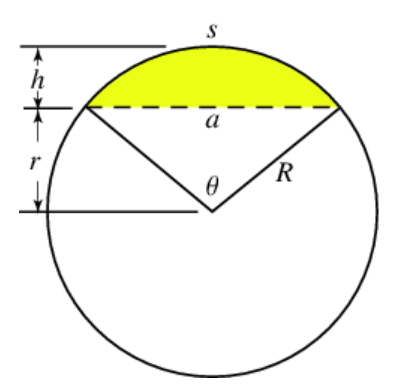
\includegraphics[scale=0.5]{math/img/circ_seg.png}
\end{center}

Radius: $R = r + h$

Arc length: $s = R \theta$

Height: $r = R \cos(\frac{1}{2} \theta) = \frac{1}{2} a \cot(\frac{1}{2} \theta) = \frac{1}{2} \sqrt{4 R^2 - a^2}$

Chord length: $a = 2R \sin(\frac{1}{2} \theta) = 2r \tan (\frac{1}{2} \theta) = 2 \sqrt{R^2 - r^2} = 2 \sqrt{h (2R - h)}$

Angle: $\theta = \frac{s}{R} = 2 \cos^{-1}(\frac{r}{R}) = 2 \tan^{-1}(\frac{a}{2r}) = 2 \sin^{-1}(\frac{a}{2R})$

Area: $A = \frac{1}{2} R^2 (\theta - \sin (\theta)) = \frac{1}{2} (Rs - ar) = R^2 \cos^{-1}(\frac{r}{R}) - r \sqrt{R^2 - r^2} = R^2 \cos^{-1}(\frac{R-h}{R}) - (R-h)\sqrt{2Rh - h^2}$

\textbf{Right circular cone}

Volume $= \frac{\pi r^2 h}{3}$

Lateral surface area $= \pi r \sqrt{r^2 + h^2}$

Total surface area $= Lateral + \pi r^2$

\textbf{Sphere}

Volume $= \frac{4}{3} \pi r^3$

Surface area $= 4 \pi r^2$

\textbf{General polygons}

Number the vertexes of the polygon, going either clockwise or counterclockwise.

$$\text{Area } = \Bigg\lvert \frac{(x_1 y_2 - y_1 x_2) + (x_2 y_3 - y_2 x_3) + ... + (x_n y_1 - y_n x_1)}{2} \Bigg\rvert$$

\subsection*{Permutations and combinations}

Combinations, no repetition: $\displaystyle \binom{n}{k} = \frac{n!}{k! (n-k)!}$

Combinations, with repetition: $\displaystyle \binom{n + k - 1}{k} = \frac{(n+k-1)!}{k! (n-1)!}$

Permutations, no repetition: $\displaystyle \frac{n!}{(n-k)!}$

Permutations, with repetition: $n^k$

\subsection*{Trigonometry}

\textbf{Law of Sine}

Use with $A, B, a$ (AAS), $A, c, B$ (ASA), and $a, b, A$ (SSA)

$$\frac{a}{\sin(A)} = \frac{b}{\sin(B)} = \frac{c}{\sin(C)} \formsep h = b \sin(A)$$

Ambiguous case: two sides and an angle \textit{not} between

\begin{itemize}
    \item Case 1: $\theta > 90^\circ$
    \begin{itemize}
        \item $opposite < adjacent$: no possible triangles
        \item $opposite > adjacent$: 1 possible triangle
    \end{itemize}
    \item Case 2: $\theta < 90^\circ$
    \begin{itemize}
        \item $opposite = height$: 1 possible right triangle
        \item $opposite < height$: no possible triangles
        \item $opposite > height$:
        \begin{itemize}
            \item $opposite < adjacent$: 1 possible triangle
            \item $opposite > adjacent$: 2 possible triangles
        \end{itemize}
    \end{itemize}
\end{itemize}

\subsection*{Law of Cosine}

Use with $a, C, b$ (SAS) and $a, b, c$ (SSS)

Note: Find the largest angle first. Find the smallest angle second. (This includes given angles. eg. if you are given SAS, find the smallest angle.)

$$a^2 = b^2 + c^2 - 2bc \cos(A)$$

\newpage
\startsection{GCD, LCM, and EEA}

\textbf{Greatest Common Divisor}

Finds the greatest common divisor:

\lstinputlisting{math/code/gcdlcmeea1.java}

Alternatively:

\lstinputlisting{math/code/gcdlcmeea2.java}

\textbf{Least Common Multiple}

$$LCM(a, b) = \frac{ab}{GCD(a, b)}$$

\subsection*{Extended Euclidean Algorithm}

\textbf{Bezout's identity}: $ax + by = d$, where $a$ and $b$ are non-zero integers, $d$ is their GCD, and $x$ and $y$ are Bezout's coefficients.

\lstinputlisting{math/code/gcdlcmeea3.java}

The "quotients by the GCD" are a and b divided by the GCD. They may have an incorrect sign. Similarly, if either a or b is zero and the other is negative, the greatest common divisor that is output is negative, and all the signs of the output must be changed.

\subsection*{Misc}

Problem: Given the equation $ax + by = c$ and the values of a, b, and c, determine if there exists a solution for x and y. \\
\indent Solution: x and y exist if c is divisible by the GCD of a and b, because it means that a, b, and c are multiples of the same number.

Problem: Given the equation $ax - by = 0$, find x and y. \\
\indent Solution: x = b / GCD and y = a / GCD. The GCD is the largest common factor they share, so A * (B/gcd) = B * (A/gcd).

\newpage
\startsection{Matrices}

Formatting: a $n \times m$ matrix is a matrix with $n$ rows and $m$ columns.

Terminology:\\
Square matrix: a $n \times n$ matrix

A matrix \textit{mod} m is just a matrix in which every number has been \textit{mod}ded by m. When doing this with matrix multiplication, add \inline{sum \%= m;} after line \#6.

The identity matrix is a $n \times n$ matrix where the elements on the main diagonal (top-left to bottom-right) are ones and the rest are zeroes. It is similar to the number 1 in numerical mathematics. 

\subsection*{Addition and subtraction}

Add/subtract each number to its pair in the second matrix. (Note: the matrices must be the same size.)

\begin{equation*}
    \begin{bmatrix}
        2 & 6 & 12 \\
        7 & -4 & 10
    \end{bmatrix}
    +
    \begin{bmatrix}
        15 & -44 & -3 \\
        8 & 0 & 9
    \end{bmatrix}
    =
    \begin{bmatrix}
        17 & -38 & 9 \\
        15 & -4 & 19
    \end{bmatrix}
\end{equation*}

\subsection*{Scalar multiplication}

Multiply every number in the matrix by the scale factor.

\begin{equation*}
    2 * 
    \begin{bmatrix}
        4 & 0 \\
        1 & -9
    \end{bmatrix}
    =
    \begin{bmatrix}
        8 & 0 \\
        2 & -18
    \end{bmatrix}
\end{equation*}

\subsection*{Multiplication (dot product)}

To get the number in row i and column j of the resulting matrix, we multiply each number in row i of the first matrix by each number in column j of the second and add the products.

If C = AB, for an $n \times m$ matrix A and an $m \times p$ matrix B, then C is an $n \times p$ matrix. Note that the number of columns in matrix A and the number of rows in matrix B must be the same.

To find A $\cdot$ B:

\lstinputlisting{math/code/matrices1.java}

\subsection*{Exponentiation}

Matrix exponentiation is essentially the same as numerical exponentiation, and can be used with fast-expo techniques. Note that raising a matrix to the zeroth power returns the identity matrix and that the matrix must be square.

\lstinputlisting{math/code/matrices2.java}

\newpage
\startsection{Miscellaneous}

\subsection*{Bell numbers} 

The number of partitions a set of n elements has. (Partition of a set: grouping of the set's elements into non-empty subsets, in such a way that every element is included in one and only one of the subsets.)

$B = \{1, 1, 2, 5, 15, 52, 203, 877, 4140, 21147, 115975, 678570, 4213597, 27644437, 190899322, 1382958545\}$

$$B_{n+1} = \sum^n_{k=0} \binom{n}{k} B_k \formsep B_n = \sum^n_{k=0} \genfrac{\{}{\}}{0pt}{}{n}{k}$$

The Bell numbers can be calculated with the Bell triangle (similar to Pascal's triangle), where B\subscript{n} is the first number in the n\textsuperscript{th} row.

\begin{center}
    \begin{tabular}{l}
    1\\
    1 2\\
    2 3 5\\
    5 7 10 15\\
    15 20 27 37 52\\
    \end{tabular}
\end{center}

\lstinputlisting{math/code/misc_bell1.java}

\subsection*{Catalan numbers}

The only Catalan numbers $C_n$ that are odd are those for which $n=2^k-1$. All others are even.

The only prime Catalan numbers are $C_2=2$ and $C_3=5$.

$C = \{1, 1, 2, 5, 14, 42, 132, 429, 1430, 4862, 16796, 58786, 208012, 742900, 2674440, 9694845, 35357670\}$

$$
    C_n = \frac{1}{n+1}\binom{2n}{n} = \binom{2n}{n} - \binom{2n}{n+1} = \frac{(2n)!}{(n+1)!n!} = \prod_{k=2}^{n} \frac{n+k}{k} = \frac{1}{n+1}\sum_{i=0}^{n}\binom{n}{i}^2 = \int_{0}^{4}x^n\frac{1}{2\pi}\sqrt{\frac{4-x}{x}} dx
$$
$$C_0 = 1 \formsep C_{n+1} = \sum_{i=0}^{n}C_i C_{n-i} = \frac{2(2n + 1)}{n+2}C_n$$

\subsection*{Coupon collector's problem}

Suppose there is an urn with n different coupons. What is the probability that more than $t$ sample trials are needed to collect all n coupons? Or, given n coupons, how many coupons do you expect you need to draw with replacement before having drawn each coupon at least once? Alternatively, how many times do you expect to need to roll an $n$-sided die in order to have every number come up at least once?

The answer: $n H_n$, where $n$ is the number of coupons and $H_n$ is the n\textsuperscript{th} Harmonic number.

$$H_n = 1 + \frac{1}{2} + \frac{1}{3} + ... + \frac{1}{n} = \sum_{k=1}^n \frac{1}{k}$$

\subsection*{Digital root formula}

The digital root of a non-negative $n$ is the result of repeatedly summing the digits of $n$. Eg. the digital root of 65,536 is 7 because $dr(65536) = 6+5+5+3+6 = 25$ and $dr(25) = 2+5 = 7$. 

$dr(n) = 1 + ((n-1) \text{ mod } 9)$. To generalize to another base $b$, change $9$ to $b-1$.

\subsection*{Double equality}

It can be hard to check equality in doubles due to floating point errors. This method will check for equality if floating point errors are possible:

\lstinputlisting{math/code/misc_doubleequal1.java}

10\textsuperscript{-9} is generally a good value for \inline{EPSILON}. Also, most problems involving doubles will tell you how much error two values can have and still be considered equal.

\subsection*{Evaluating polynomials at a point}

Given an array of the coefficients of a polynomial you can find the value of the polynomial evaluated at \inline{x} (ie. $f(x)$). This works by the remainder theorem.

\lstinputlisting{math/code/misc_evalpoly1.java}

Note that the array of coefficients should be in descending order. If \inline{P(x) = 3x\textsuperscript{2} - 2x + 1}, then the array should equal \inline{\{3, -2, 1\}}.

\subsection*{Fibonacci sequence}

$F = \{0, 1, 1, 2, 3, 5, 8, 13, 21, 34, 55, 89, 144, 233, 377, 610\}$

If $5x^2 + 4$ or $5x^2 - 4$ is a perfect square, then x is part of the Fibonacci sequence.

Every 3\textsuperscript{rd} number of the sequence is even and more generally, every k\textsuperscript{th} number of the sequence is a multiple of F\subscript{k}. In fact, it satisfies the stronger divisibility property $GCD(F_m, F_n) = F_{GCD(m, n)}$.

Any three consecutive Fibonacci numbers are pairwise coprime, ie. $GCD(F_n, F_{n+1}) = GCD(F_n, F_{n+2}) = GCD(F_{n+1}, F_{n+2}) = 1$.

Every prime number $p$ divides a Fibonacci number that can be determined by the value of $p \mymod{5}$. If p is congruent to 1 or 4 (mod 5), then $p$ divides F\subscript{p-1}, and if p is congruent to 2 or 3 (mod 5), then, p divides F\subscript{p+1}. The remaining case is that $p = 5$, and in this case $p$ divides F\subscript{p}.

You can use matrices to calculate the Fibonacci sequence. This matrix representation gives the following closed expression for the Fibonacci numbers:

\begin{equation*}
    \begin{bmatrix}
        F_{n+1} & F_n \\
        F_n & F_{n-1}
    \end{bmatrix}
    =
    \begin{bmatrix}
        1 & 1 \\
        1 & 0
    \end{bmatrix}
    ^n
    \formsep
    \begin{bmatrix}
        F_n \\
        F_{n-1}
    \end{bmatrix}
    =
    \begin{bmatrix}
        1 & 1 \\
        1 & 0
    \end{bmatrix}
    \begin{bmatrix}
        F_{n-1} \\
        F_{n-2}
    \end{bmatrix}
\end{equation*}

\textbf{Generalization}

If $F_0 = a$ and $F_1 = b$, then:

\begin{equation*}
    \begin{bmatrix}
        F_n \\
        F_{n-1}
    \end{bmatrix}
    =
    \begin{bmatrix}
        1 & 1 \\
        1 & 0
    \end{bmatrix}
    ^{n-1}
    \begin{bmatrix}
        b \\
        a
    \end{bmatrix}
\end{equation*}

If $a = b = 1$, then the Fibonacci sequence will be "shifted" to the left by one. For example, 8 is the 6\textsuperscript{th} Fibonacci number, but would be the 5\textsuperscript{th} in the generalized Fibonacci sequence.

(If $a = 0$ and $b = 1$, then it will be the normal sequence.)

\subsection*{Finding the average of two values}

Obviously, you can do it like this: \inline{int c = (a + b) >> 1;}

However, that can lead to overflows. This will not: \inline{int c = a + ((b - a) >> 1);}

Alternatively: \inline{((x $\wedge$ y) >> 1) + (x \& y)}

\subsection*{Log properties}

$$log_b(x) = \frac{log_y(x)}{log_y(b)} \text{, where } y \text{ is any base}$$

\subsection*{Pascal's triangle}

\begin{center}
1 \\
1 1 \\
1 2 1 \\
1 3 3 1 \\
1 4 6 4 1 \\
1 5 10 10 5 1
\end{center}

Pascal’s triangle is a triangular array of the binomial coefficients, that is $(x + y)^n$. The rows (designated by $n$) and columns (designated by $k$) are 0-indexed. So 6 is at row 4, column 2. This is also known as \textit{n choose k} or $\binom{n}{k}$.

\lstinputlisting{math/code/misc_pascal1.java}

Given the n\textsuperscript{th} row of Pascal's triangle (in \inline{coefficients}) and values of a and b (from the expression $(ax + by)^{pow}$), this will give you the coefficients of the expanded binomial expression.

\lstinputlisting{math/code/misc_pascal2.java}

\subsection*{Pigeonhole principle}

The pigeonhole principle states that if $k$ objects are placed into $n$ boxes, then at least one box must hold at least $\lceil \frac{n}{k} \rceil$ objects.

\subsection*{Primality}

This is a longer isPrime method, but one that is faster than the “na\"{\i}ve version.

\lstinputlisting{math/code/misc_primality1.java}

\subsection*{Prime factorization}

This finds all the prime factors (and not non-prime factors) because of the same principle as the prime sieve.

\lstinputlisting{math/code/misc_primefact1.java}

\subsection*{Pythagorean triple}

A Pythagorean Triple is 3 numbers, a, b, c, such that $a^2 + b^2 = c^2$. For all Pythagorean Triples, there exist positive integers x and y, with x $>$ y, such that:
$$a = x^2 - y^2 \formsep b = 2xy \formsep c = x^2 + y^2$$

\subsection*{Stirling numbers (second kind)}

The number of ways to partition a set of n distinguishable objects into k non-empty subsets (denoted $S(n, k)$ or $\genfrac{\{}{\}}{0pt}{}{n}{k}$).
$$S(n, k) = S(n-1, k-1) + k*S(n-1, k) = \frac{1}{k!} \sum_{j=0}^k (-1)^{k-j} \binom{k}{j} j^n$$

\begin{center}
    \begin{tabular}{|c|c|c|c|c|c|c|c|c|c|c|c|}
        \hline
        n / k & 0 & 1 & 2 & 3 & 4 & 5 & 6 & 7 & 8 & 9 & 10 \\
        \hline
        0 & 1 & & & & & & & & & & \\
        \hline
        1 & 0 & 1 & & & & & & & & & \\
        \hline
        2 & 0 & 1 & 1 & & & & & & & & \\
        \hline
        3 & 0 & 1 & 3 & 1 & & & & & & & \\
        \hline
        4 & 0 & 1 & 7 & 6 & 1 & & & & & & \\
        \hline
        5 & 0 & 1 & 15 & 25 & 10 & 1 & & & & & \\
        \hline
        6 & 0 & 1 & 31 & 90 & 65 & 15 & 1 & & & & \\
        \hline
        7 & 0 & 1 & 63 & 301 & 350 & 140 & 21 & 1 & & & \\
        \hline
        8 & 0 & 1 & 127 & 966 & 1701 & 1050 & 266 & 28 & 1 & & \\
        \hline
        9 & 0 & 1 & 255 & 3025 & 7770 & 6951 & 2946 & 462 & 36 & 1 & \\
        \hline
        10 & 0 & 1 & 511 & 9330 & 34105 & 42525 & 22827 & 5880 & 750 & 45 & 1 \\
        \hline
    \end{tabular}
\end{center}

The sum over the values for k of the Stirling numbers of the second kind, gives us $\displaystyle B_n = \sum_{k=0}^n \genfrac{\{}{\}}{0pt}{}{n}{k}$, ie. the n\textsuperscript{th} Bell number.

\subsection*{Stirling's approximation}

$$\text{ln}(n!) \approx n \text{ln}(n) - n \formsep n! \approx \sqrt{2 \pi n} \bigg(\frac{n}{e} \bigg)^n$$

\newpage
\startsection{Sieves}

\subsection*{Sieve of Eratosthenes}

\textit{Runtime: O(n log(log(n)))}

The Sieve of Erastosthenes computes primes by “marking off” multiples of all the primes before the current prime. The limit of how large a number you can check with this is based on how large an array you can make. However, you can “double” the max number by using a Sieve that only checks odd numbers. If you need a really large sieve, use a BitSet.

\lstinputlisting{math/code/sieves1.java}

You can count the number of prime factors a number has by changing lines 5-7 to:

\lstinputlisting{math/code/sieves2.java}

(A number i is prime if \inline{numPrimeFactors[i]} is 0.)

\subsection*{Totient sieve}

This can also be used as a prime sieve, because \inline{p} is prime if \inline{phi[p] == p-1}.

\lstinputlisting{math/code/sieves3.java}

\subsection*{Mod inverse sieve}

The modular inverse of \inline{i} \textit{mod} \inline{m}.

\lstinputlisting{math/code/sieves4.java}

\newpage

\end{document}
